\documentclass[10pt]{article}

\usepackage[margin=0.72in]{geometry}
\usepackage{times}
\usepackage{graphicx}
\usepackage{amsmath}
\usepackage{booktabs}
\usepackage[hidelinks]{hyperref}
\usepackage{enumitem}
\usepackage{placeins}

\graphicspath{{../artifacts/paper_assets_20260613/}}
\setlist{nosep,leftmargin=*}
\setlength{\parskip}{0.28em}
\setlength{\parindent}{0pt}

\title{\vspace{-1.2em}GeoNexus-RSD: Hierarchy- and Context-Aware Vision-Language Prompting for Oriented Remote Sensing Detection}
\author{
Dinghao Li\\
Xi'an Jiaotong University\\
\texttt{lidinghao@xjtu.stu.cn}
}
\date{}

\begin{document}
\maketitle
\vspace{-1.4em}

\begin{abstract}
Oriented object detection in remote sensing images must distinguish small, dense, and semantically similar targets under large scale variation and arbitrary rotation. We study GeoNexus-RSD, a detector-centered vision-language prompting framework that augments a strong oriented detector with taxonomy-aware class prompts, hierarchy regularization, scene/context adaptation, and conservative pseudo-label purification. The current route is DOTA2-first: DOTA2 is the primary benchmark, DIOR-R is the required cross-dataset validation, and FAIR1M is reserved for later fine-grained evidence. As of 2026-06-13, the completed GeoNexus DOTA2 S1 run reaches 0.6177 mAP and 0.6180 AP50 on \texttt{DOTA2\_1024\_500/ss\_val}, improving over the matched RoI Transformer S0 baseline of 0.6088/0.6090. Seven DOTA2 S2 loss-0 runs show repeatable best-checkpoint signal with mean 0.620606, but final checkpoints average 0.616655 and remain unstable. On sanitized DIOR-R, RoI Transformer S0 reaches 0.6531/0.6530 and two S1 replicas reach 0.6751/0.675 and 0.6690/0.669, while S2 hierarchy replicas have clean startup but pending metrics. The draft therefore reports current evidence conservatively: measured DOTA2 and DIOR-R results are separated from active, planned, paused, and archive-only evidence.
\end{abstract}

\section{Introduction}

Remote sensing object detection supports transportation monitoring, maritime surveillance, urban analytics, disaster assessment, and defense-oriented interpretation. Compared with natural-image detection, aerial scenes contain very large images, dense object layouts, long-tail categories, strong scale variation, and objects with arbitrary orientation. DOTA made rotated object detection a standard benchmark for such imagery \cite{xia2018dota}. Strong oriented detectors such as RoI Transformer, Oriented R-CNN, ReDet, and Oriented RepPoints improve the geometric path through transformed RoIs, oriented proposals, rotation-equivariant features, or point-set representations \cite{ding2019roit,xie2021orientedrcnn,han2021redet,li2022orientedreppoints}.

Most oriented detectors still treat categories as independent closed-set labels. This is limiting for remote sensing. Fine-grained targets share local appearance, class definitions vary across datasets, and the same visual crop may need surrounding context to disambiguate. A bright elongated region may be a small vehicle, a ship, a harbor structure, or part of an airport scene depending on nearby roads, water, or facilities. Language-aligned models provide a path for adding semantic priors without abandoning standard detector protocols.

GeoNexus-RSD keeps the detector backbone and oriented-box protocol central, then injects structured semantic evidence through prompts. The core modules are:
\begin{itemize}
\item a hierarchical prompt bank grounded in class names, aliases, parent categories, and confusing class pairs;
\item a prompt-conditioned classification path using real RemoteCLIP text embeddings where available;
\item a hierarchy regularizer that penalizes semantically inconsistent class scores;
\item a scene/context adapter and pseudo-label purification stage, both kept paused until DOTA2 S1/S2 and DIOR-R become stable.
\end{itemize}

This draft is not a final submission. It is a stronger paper draft and evidence ledger for the DOTA2-first route. Its contribution is to define the method, record the present measured evidence, show publication-style figures and tables, and make unsupported items explicit.

\section{Related Work}

\textbf{Oriented remote sensing detection.}
DOTA established a large-scale aerial object benchmark with oriented boxes and dense object layouts \cite{xia2018dota}. RoI Transformer learns rotated RoIs from horizontal proposals \cite{ding2019roit}. Oriented R-CNN simplifies the two-stage oriented detection pipeline with oriented proposals \cite{xie2021orientedrcnn}. ReDet introduces rotation-equivariant feature extraction for aerial scenes \cite{han2021redet}. Oriented RepPoints models oriented objects through adaptive point sets \cite{li2022orientedreppoints}. GeoNexus-RSD follows this detector family and asks whether structured language evidence can improve classification behavior while preserving the same oriented-box evaluation protocol.

\textbf{Vision-language detection and remote sensing prompts.}
CLIP-style pretraining aligns visual and language representations at scale \cite{radford2021clip}. GLIP, RegionCLIP, and Detic extend language supervision to detection \cite{li2022glip,zhong2022regionclip,zhou2022detic}. Remote sensing transfer is difficult because aerial targets are small, rotated, and often context-dependent. RemoteCLIP, SkyScript, and GeoRSCLIP motivate remote-sensing-specific image-text alignment \cite{remoteclip2023,skyscript2023,georsclip2023}. OpenRSD is the closest reference direction for open-prompt remote sensing detection \cite{huang2025openrsd}. GeoNexus-RSD uses this literature to motivate prompt structure but does not claim open-vocabulary detection unless a real open-vocabulary or vocabulary-robustness evaluation is run.

\textbf{Pseudo-label denoising.}
Unbiased Teacher and Soft Teacher show that pseudo labels can improve detection when noise is controlled \cite{liu2021unbiased,xu2021softteacher}. Remote sensing pseudo labels are fragile because small objects, dense duplicates, and ambiguous categories create false positives and class swaps. SemiEarth motivates vision-language purification in remote sensing \cite{semiearth2026}. GeoNexus-RSD adapts this idea to oriented detection only as a planned stage until DOTA2 S1/S2 and DIOR-R are stable.

\section{Method}

Given an aerial tile $I$, an oriented detector predicts rotated boxes $b_i=(x_i,y_i,w_i,h_i,\theta_i)$ and class scores over vocabulary $\mathcal{C}$. GeoNexus-RSD keeps the detector-native geometric branch and adds a semantic branch based on a taxonomy $\mathcal{T}$ over $\mathcal{C}$. Figure~\ref{fig:framework} shows the detector-style architecture.

\begin{figure}[t]
\centering

\includegraphics[width=0.98\linewidth]{fig_method_framework_tikz.pdf}
\caption{GeoNexus-RSD detector/prompt architecture. The detector geometry path and S1 prompt path are implemented paper-facing modules; S2 is an early-checkpoint candidate with unstable finals; context gating and pseudo-label purification remain paused or planned until the DOTA2 and DIOR-R gates are stable.}
\label{fig:framework}
\end{figure}

\subsection{Hierarchical Prompt Bank}

For each class $c\in\mathcal{C}$, the prompt bank stores class names, aliases, parent descriptors, scene descriptors, and contrastive phrases:
\begin{equation}
    \mathcal{P}_c=\{p_{c,1},\ldots,p_{c,K}\}, \qquad e_{c,k}=T(p_{c,k}).
\end{equation}
The class embedding is a weighted prompt mixture:
\begin{equation}
    \bar{e}_c=\sum_{k=1}^{K}\alpha_{c,k}e_{c,k}, \qquad \sum_{k=1}^{K}\alpha_{c,k}=1.
\end{equation}
In the current DOTA2 and DIOR-R routes, RemoteCLIP ViT-B/32 provides real text embeddings. The DOTA2 S2 prompt artifact contains 18 finite, normalized class embeddings and an $18\times18$ relation matrix; the DIOR-R S2 artifact contains 20 finite, normalized class embeddings and a $20\times20$ relation matrix. This matters because the evidence should not be described as VLM-based if a run falls back to deterministic hash embeddings.

\subsection{Hierarchy Regularization}

The taxonomy supplies parent-child and related-category edges $\mathcal{E}_{\mathcal{T}}$. A simple margin regularizer penalizes inconsistent score orderings:
\begin{equation}
    \mathcal{L}_{hier}=
    \sum_{(u,v)\in\mathcal{E}_{\mathcal{T}}}
    \max(0, s_v-s_u+m),
\end{equation}
where $s_u$ and $s_v$ are prompt-conditioned scores and $m$ is a margin. The term is designed for fine-grained aerial classes where errors often occur inside semantically related groups such as vehicle-like, ship/harbor, or airport/helipad categories. The DOTA2 S2 loss-0 stabilization runs show a best-checkpoint mean above S1 but final-checkpoint instability, so the present draft treats S2 as an early-checkpoint candidate rather than a final improvement. DIOR-R S2 hierarchy replicas have clean startup and pending metrics.

\subsection{Scene Context Adapter}

Let $F(I)$ be the detector feature map, $g=\mathrm{GAP}(F(I))$ a tile descriptor, and $r_i$ a region feature. The context-adapted class embedding is:
\begin{equation}
    \tilde{e}_{c,i}=\bar{e}_c + A([g,r_i,\bar{e}_c]),
\end{equation}
where $A(\cdot)$ is a lightweight adapter. The prompt-conditioned classification logit is:
\begin{equation}
    z_{i,c}=\tau^{-1}
    \frac{\phi(r_i)^{\top}\psi(\tilde{e}_{c,i})}
    {\|\phi(r_i)\|_2\|\psi(\tilde{e}_{c,i})\|_2}.
\end{equation}
The box regression branch remains detector-native. This keeps localization comparable to standard oriented baselines. The context adapter is a core method component, but it remains paused as a paper-facing experiment until DOTA2 S2 and DIOR-R are stable.

\subsection{Pseudo-Label Purification}

For a candidate pseudo box $\hat{b}_j$ with class $\hat{c}_j$, the planned purification score is:
\begin{equation}
    q_j=\sigma(\beta_1 d_j+\beta_2 h_j+\beta_3 v_j+\beta_4 a_j),
\end{equation}
where $d_j$ is detector confidence, $h_j$ hierarchy consistency, $v_j$ crop-text agreement, and $a_j$ geometric plausibility. Accepted pseudo labels are weighted softly:
\begin{equation}
    \mathcal{L}=\mathcal{L}_{det}^{sup}
    +\lambda_h\mathcal{L}_{hier}
    +\lambda_p\sum_j q_j\left(
    \mathcal{L}_{cls}^{pseudo}(j)+\lambda_b\mathcal{L}_{box}^{pseudo}(j)\right).
\end{equation}
This stage is part of the intended GeoNexus-RSD design but is not yet completed evidence.

\section{Experimental Route and Evidence}

\subsection{DOTA2-First Route}

DOTA2 is the primary benchmark. The current matched S0 detector is RoI Transformer on \texttt{DOTA2\_1024\_500/ss\_val} after valid-PNG recovery. The paper-facing positive result is one completed GeoNexus S1 run initialized with RemoteCLIP prompts. Figure~\ref{fig:route} separates measured DOTA2 and DIOR-R evidence from unstable, pending, paused, and archive-only evidence.

\begin{figure}[t]
\centering
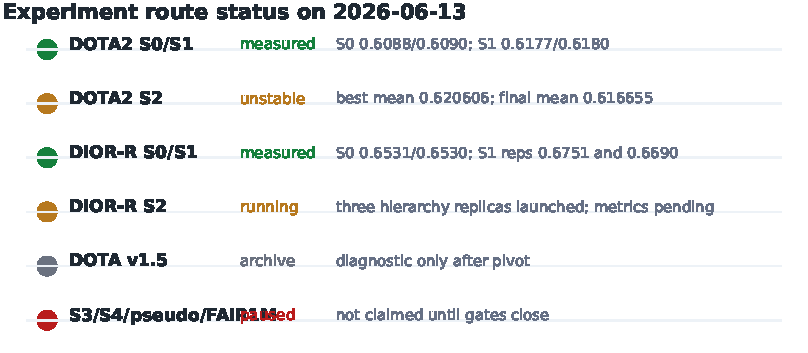
\includegraphics[width=0.98\linewidth]{fig_route_status.pdf}
\caption{Experiment route/status figure. DOTA2 and DIOR-R measured results are separated from unstable S2 finals, pending DIOR-R S2 replicas, archive-only DOTA v1.5 diagnostics, and paused S3/S4, pseudo-label, routing, and FAIR1M work.}
\label{fig:route}
\end{figure}

\begin{table}[t]
\centering
\small
\caption{DOTA2 evidence after the June 13 S2 stabilization analysis.}
\label{tab:dota2_current}
\begin{tabular}{lllrl}
\toprule
Run & Status & mAP & AP50 & Use \\
\midrule
DOTA2 S0 RoI Transformer & complete & 0.6088 & 0.6090 & matched valid-PNG detector baseline \\
DOTA2 S1 RemoteCLIP & complete & 0.6177 & 0.6180 & paper-facing positive DOTA2 result \\
DOTA2 S2 loss-0 best mean & candidate & 0.620606 & - & all-seven best-checkpoint mean; early only \\
DOTA2 S2 loss-0 final mean & unstable & 0.616655 & - & all-seven final mean; below S1 \\
\bottomrule
\end{tabular}
\end{table}


The headline DOTA2 interpretation is narrow. GeoNexus S1 GPU-1 improves over the matched RoI Transformer S0 baseline by 0.0089 mAP and 0.0090 AP50. The S2 loss-0 stabilization set is stronger when selecting best checkpoints, with all-seven best mean 0.620606, but final checkpoints average 0.616655 and fall below S1. Therefore S2 supports an early-checkpoint candidate, not a completed final-epoch stability claim.

\begin{figure}[t]
\centering
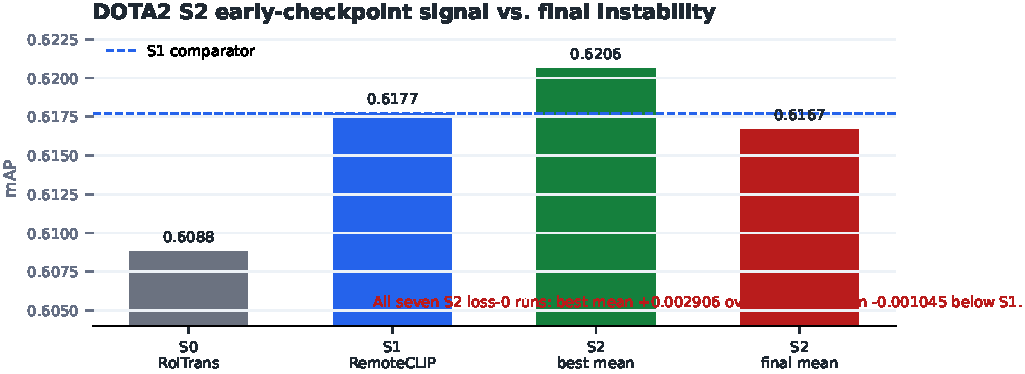
\includegraphics[width=0.98\linewidth]{fig_dota2_s2_stability.pdf}
\caption{DOTA2 S2 stability chart. S2 best checkpoints are above S1 on average, but final checkpoints remain unstable and should not be cited as final S2 evidence.}
\label{fig:dota2_rank}
\end{figure}

\begin{figure}[t]
\centering
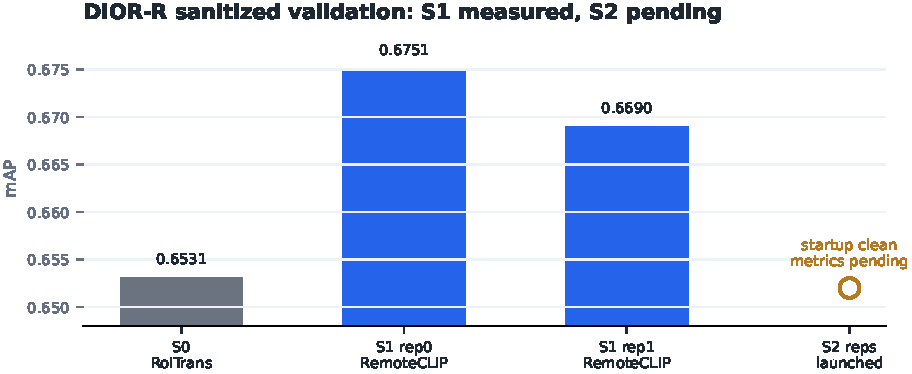
\includegraphics[width=0.98\linewidth]{fig_dior_r_transfer.pdf}
\caption{DIOR-R sanitized transfer evidence. RoI Transformer S0 is the current DIOR-R detector baseline, two RemoteCLIP S1 replicas are measured, and S2 hierarchy replicas are launched with clean startup but pending metrics.}
\label{fig:dior_transfer}
\end{figure}

\subsection{Class-Level and Visual Evidence}

The current draft includes class-level S0 evidence as appendix-style diagnostic context. Real qualitative detections and accepted/rejected pseudo-label examples must be added only after valid inference artifacts are archived.

\begin{figure}[t]
\centering

\includegraphics[width=0.98\linewidth]{fig_dota2_class_heatmap.pdf}
\caption{DOTA2 S0 class evidence groups generated from the RoI Transformer valid-PNG metric record. This is diagnostic context for prompt design and confusing-class analysis.}
\label{fig:class}
\end{figure}

\subsection{GeoNexus Stage Ablation Status}

\begin{table}[t]
\centering
\small
\caption{Route status used to prevent overclaiming active or paused modules.}
\label{tab:route_status}
\begin{tabular}{lll}
\toprule
Track & Role & Status \\
\midrule
DOTA2 & primary benchmark & S0/S1 measured; S2 best-checkpoint candidate \\
DIOR-R & required validation & S0/S1 measured; S2 metrics pending \\
DOTA v1.5 & archive only & diagnostic history, not headline evidence \\
S3/S4 & paused & resume only after S2 and DIOR-R gates are stable \\
Pseudo-label / FAIR1M & planned & no paper-facing metric claim yet \\
\bottomrule
\end{tabular}
\end{table}


Table~\ref{tab:route_status} intentionally mixes measured route points with pending/paused rows, but each row is marked by role and status. DOTA v1.5 rows are archive diagnostics and must not be used as headline benchmark evidence after the 2026-06-06 pivot.

\subsection{DIOR-R Diagnostic Gate}

DIOR-R is required for cross-dataset validation. The earlier NaN/Inf detector path was addressed through sanitized-label scans and bounded train-step diagnostics. The current sanitized RoI Transformer S0 reaches 0.6531/0.6530, and RemoteCLIP S1 replicas reach 0.6751/0.675 and 0.6690/0.669. DIOR-R S2 hierarchy replicas have clean startup, but their metrics are pending and must not be reported as gains.

\begin{table}[t]
\centering
\small
\caption{DIOR-R sanitized route evidence and pending S2 status.}
\label{tab:dior_r_current}
\begin{tabular}{lllrl}
\toprule
Run & Status & mAP & AP50 & Use \\
\midrule
DIOR-R S0 RoI Transformer & sanitized S0 & 0.6531 & 0.6530 & current S0 leader \\
DIOR-R S1 rep0 & complete & 0.6751 & 0.675 & stronger S1 replica; source for S2 \\
DIOR-R S1 rep1 & complete & 0.6690 & 0.669 & stability replica \\
DIOR-R S2 hierarchy reps & launched & pending & pending & clean startup; no metric claim \\
\bottomrule
\end{tabular}
\end{table}


\subsection{Prompt and Reporting Tables}

\begin{table}[t]
\centering
\small
\caption{Source map for the June 13 generated paper assets.}
\label{tab:artifact_sources}
\begin{tabular}{lll}
\toprule
Claim & Value & Local source \\
\midrule
DOTA2 S0 & 0.6088 / 0.6090 & docs/experiments/20260603\_s0\_dota2\_roi\_trans\_validpng\_metrics.json \\
DOTA2 S1 & 0.6177 / 0.6180 & docs/experiments/20260608\_dota2\_s1\_complete\_and\_s2\_launch.md \\
DOTA2 S2 aggregate & best 0.620606; final 0.616655 & docs/experiments/20260611\_dota2\_s2\_loss0\_replicates\_analysis.md \\
DIOR-R S0 & 0.6531 / 0.6530 & docs/experiments/20260613\_dior\_r\_s0\_sanitized\_long\_interim.md \\
DIOR-R S1 replicas & 0.6751 / 0.675; 0.6690 / 0.669 & docs/experiments/20260613\_dior\_r\_geonexus\_s1\_s0e52\_replicas\_metrics.json \\
DIOR-R S2 & startup clean; metrics pending & docs/experiments/20260613\_dior\_r\_geonexus\_s2\_hierarchy\_replicas\_launch.md \\
\bottomrule
\end{tabular}
\end{table}


The final paper must still add measured parameters, memory, latency, and FLOPs, or omit efficiency claims entirely.

\subsection{Archive-Only DOTA v1.5 Diagnostics}

DOTA v1.5 GeoNexus experiments exercised the hierarchy and context code paths, but they are no longer the formal benchmark route. They should remain in experiment records and may be used for debugging narratives, not as headline table evidence. Any final paper table must keep DOTA v1.5 separate from DOTA2 and DIOR-R.

\begin{table}[t]
\centering
\small
\caption{Archive-only DOTA v1.5 reduced tiled diagnostics. These values are not headline evidence.}
\label{tab:archive}
\begin{tabular}{llll}
\toprule
Stage & Setting & Best & Final \\
\midrule
S0 & RoI Transformer 3x baseline & 0.2644 / 0.2640 & 0.2612 / 0.2610 \\
S1 & RemoteCLIP prompt head & 0.2666 / 0.2670 & 0.2506 / 0.2510 \\
S2 & Hierarchy regularizer 72e & 0.3757 / 0.3760 & 0.3738 / 0.3740 \\
S3 & Scene adapter 72e & 0.3800 / 0.3800 & 0.3759 / 0.3760 \\
\bottomrule
\end{tabular}
\end{table}

\section{Required Final Analyses}

The final submission should contain only measured rows. The current draft records the required analysis set so that future work can close the evidence gaps without shifting the story.

\begin{table}[t]
\centering
\small
\caption{Required final analyses. Planned rows must be replaced by measured values before submission.}
\label{tab:protocol}
\begin{tabular}{lll}
\toprule
Analysis & Required datasets & Purpose \\
\midrule
Main comparison & DOTA2, DIOR-R & Compare S0 detector and GeoNexus variants \\
Core ablation & DOTA2, DIOR-R & Isolate prompt bank, hierarchy, and context modules \\
Prompt robustness & DOTA2 & Compare labels, aliases, parents, and mixed prompts \\
Pseudo-label quality & DOTA2, DIOR-R when stable & Measure accepted/rejected pseudo-label precision \\
Efficiency & DOTA2 & Report parameters, memory, latency, and FLOPs per tile \\
Qualitative evidence & DOTA2, DIOR-R & Show valid detections and failure cases from archived inference artifacts \\
\bottomrule
\end{tabular}
\end{table}

All tables must record dataset version, split, config, checkpoint, metric source, and whether embeddings are real VLM embeddings or fallback embeddings. DOTA2 remains the primary benchmark. DIOR-R is required for cross-dataset validation. FAIR1M is a stretch dataset for fine-grained hierarchy analysis only after DOTA2 and DIOR-R are stable.

\section{Limitations and Next Steps}

The current evidence has four limitations. First, the positive DOTA2 S1 result is one completed main run, and S2 final checkpoints remain unstable despite repeatable best-checkpoint signal. Second, DIOR-R S1 is now measured on sanitized labels, but DIOR-R S2 metrics are pending. Third, the context adapter, pseudo-label purification, and FAIR1M evidence remain paused. Fourth, no measured pseudo-label quality or efficiency table is available.

The immediate next steps are:
\begin{enumerate}
\item decide a defensible DOTA2 S2 checkpoint-selection protocol or archive S2 as unstable;
\item finish and archive DIOR-R S2 hierarchy replicas;
\item compare DIOR-R S0, S1, and S2 best/final checkpoints separately;
\item keep DOTA v1.5 diagnostics out of headline benchmark tables;
\item measure efficiency and add valid qualitative detections only from archived inference artifacts.
\end{enumerate}

Only after these gates should the work advance to scene adaptation, pseudo-label purification, routing, or FAIR1M.

\section{Conclusion}

GeoNexus-RSD studies hierarchy- and context-aware vision-language prompting for oriented remote sensing detection. The current DOTA2-first evidence shows one completed GeoNexus S1 run above the matched RoI Transformer baseline, DOTA2 S2 best-checkpoint signal with unstable finals, and measured DIOR-R S1 replicas above the sanitized RoI Transformer S0 baseline. This draft therefore frames the method and evidence conservatively: DOTA2 is the primary benchmark, DIOR-R is the required validation gate, DOTA v1.5 is archive-only, and S2, pseudo-label, S3/S4, and FAIR1M outcomes are not treated as completed final evidence.

\FloatBarrier

\begin{thebibliography}{20}

\bibitem{xia2018dota}
Gui Song Xia et al.
\newblock DOTA: A Large Scale Dataset for Object Detection in Aerial Images.
\newblock In \emph{CVPR}, 2018.

\bibitem{ding2019roit}
Jian Ding, Nan Xue, Yang Long, Gui Song Xia, and Qikai Lu.
\newblock Learning RoI Transformer for Oriented Object Detection in Aerial Images.
\newblock In \emph{CVPR}, 2019.

\bibitem{xie2021orientedrcnn}
Xingxing Xie et al.
\newblock Oriented R-CNN for Object Detection.
\newblock In \emph{ICCV}, 2021.

\bibitem{han2021redet}
Jiaming Han, Jian Ding, Jie Li, and Gui Song Xia.
\newblock ReDet: A Rotation Equivariant Detector for Aerial Object Detection.
\newblock In \emph{CVPR}, 2021.

\bibitem{li2022orientedreppoints}
Wentong Li et al.
\newblock Oriented RepPoints for Aerial Object Detection.
\newblock In \emph{CVPR}, 2022.

\bibitem{huang2025openrsd}
Huang et al.
\newblock OpenRSD: Towards Open-prompts for Object Detection in Remote Sensing Images.
\newblock In \emph{ICCV}, 2025.

\bibitem{remoteclip2023}
Delong Chen et al.
\newblock RemoteCLIP: A Vision Language Foundation Model for Remote Sensing.
\newblock arXiv:2306.11029, 2023.

\bibitem{skyscript2023}
Zhecheng Wang et al.
\newblock SkyScript: A Large and Semantically Diverse Vision-Language Dataset for Remote Sensing.
\newblock arXiv:2312.12856, 2023.

\bibitem{georsclip2023}
Zilun Zhang et al.
\newblock GeoRSCLIP: A Remote Sensing Vision-Language Model.
\newblock arXiv:2306.11300, 2023.

\bibitem{semiearth2026}
SemiEarth authors.
\newblock SemiEarth: Vision Language Purified Semi Supervised Learning for Remote Sensing Semantic Segmentation.
\newblock arXiv:2602.00202, 2026.

\bibitem{radford2021clip}
Alec Radford et al.
\newblock Learning Transferable Visual Models From Natural Language Supervision.
\newblock In \emph{ICML}, 2021.

\bibitem{li2022glip}
Liunian Harold Li et al.
\newblock Grounded Language Image Pre-training.
\newblock In \emph{CVPR}, 2022.

\bibitem{zhong2022regionclip}
Yiwu Zhong et al.
\newblock RegionCLIP: Region-based Language-Image Pretraining.
\newblock In \emph{CVPR}, 2022.

\bibitem{zhou2022detic}
Xingyi Zhou et al.
\newblock Detecting Twenty-thousand Classes using Image-level Supervision.
\newblock In \emph{ECCV}, 2022.

\bibitem{liu2021unbiased}
Yen-Cheng Liu et al.
\newblock Unbiased Teacher for Semi-Supervised Object Detection.
\newblock In \emph{ICLR}, 2021.

\bibitem{xu2021softteacher}
Mengde Xu et al.
\newblock End-to-End Semi-Supervised Object Detection with Soft Teacher.
\newblock In \emph{ICCV}, 2021.

\end{thebibliography}

\end{document}
